\documentclass[11pt, openright]{book}

    % Cover Variables
    \newcommand{\ctoptitle}{}
    \newcommand{\ctitle}{CNC TECHNICAL MANUAL}
    \newcommand{\cautor}{Author}
    \newcommand{\cdate}{03.07.2024}
    \newcommand{\sectittle}{Second Title}


    % Header Variables
        \newcommand{\headRE}{Technical Manual}
        \newcommand{\headLE}{\emph{\rightmark}}
        \newcommand{\footRE}{L.Lescure A.Sionville T.Paillet $-$ \cdate}
        \newcommand{\footLE}{\emph{\thepage}}

    % TOC Variables
        \newcommand{\toctitle}{Table of Content}
        
        \newcommand{\tocchapter}{Chapter}
        \newcommand{\toccount}{2}
  
    % Chapter Variables
        \newcommand{\chvar}{Chapter -}

\usepackage[a4paper, total={16cm, 22.125cm}]{geometry}

% Page Style
\usepackage[]{environ}
% Cover Page 
\usepackage{tikz}
\makeatletter
\def\parsecomma#1,#2\endparsecomma{\def\page@x{#1}\def\page@y{#2}}
\tikzdeclarecoordinatesystem{page}{
    \parsecomma#1\endparsecomma
    \pgfpointanchor{current page}{north east}
    % Save the upper right corner
    \pgf@xc=\pgf@x%
    \pgf@yc=\pgf@y%
    % save the lower left corner
    \pgfpointanchor{current page}{south west}
    \pgf@xb=\pgf@x%
    \pgf@yb=\pgf@y%
    % Transform to the correct placement
    \pgfmathparse{(\pgf@xc-\pgf@xb)/2.*\page@x+(\pgf@xc+\pgf@xb)/2.}
    \expandafter\pgf@x\expandafter=\pgfmathresult pt
    \pgfmathparse{(\pgf@yc-\pgf@yb)/2.*\page@y+(\pgf@yc+\pgf@yb)/2.}
    \expandafter\pgf@y\expandafter=\pgfmathresult pt
}
\makeatother


% Object formatting
\usepackage[12pt]{moresize}
\usepackage[]{anyfontsize}
\usepackage{titlesec}
\usepackage{import}
\usepackage{floatrow}
\usepackage{enumitem}
\usepackage{changepage}
\usepackage[normalem]{ulem}
\usepackage{array}
\newcommand{\ul}[1]{\underline{#1}}

\usepackage[]{chngcntr}
\usepackage{ifthen}
\ifthenelse{\figcountdepth > 1}
  {\counterwithin{figure}{section}\counterwithin{table}{section}}
  {}

\usepackage[format=plain, labelfont=it, textfont=it]{caption}
\makeatletter
\def\@makecaption#1#2{%
    \vskip\abovecaptionskip
    \sbox\@tempboxa{\textit{#1.} #2}

       
   

    \ifdim \wd\@tempboxa >\hsize
        #1. #2\par
    \else
        \global \@minipagefalse
        \hb@xt@\hsize{\hfil\box\@tempboxa\hfil}
    \fi
    \vskip\belowcaptionskip}
\makeatother

\DeclareCaptionFormat{underline}{\uline{#1#2#3}\par}

% Sections
\titleformat{\section}{\fontsize{16}{19.2}\bfseries}{\thesection.}{0.25em}{}
\titleformat{\subsection}{\fontsize{14}{16.8}\bfseries}{\tab\thesubsection.}{0.25em}{}
\titleformat{\subsubsection}{\fontsize{10}{12}}{\uline{\thesubsubsection)\enspace}}{0em}{\uline}





% Geometry

% Typewritting

\setlength{\parskip}{1em}
\setlength{\parindent}{0em}


\newenvironment{items}[3][0pt]
{\def\closesep{#3}
    \vspace{#2}
    \begin{itemize}
        \setlength{\itemsep}{#1}
        \setlength{\topsep}{0pt}
        \setlength{\partopsep}{0pt}}
        {\end{itemize}
    \vspace{\closesep}}

\newenvironment{enum}[3][0pt]
{\defclosesep{#3}
    \vspace{#2}
    \begin{enumerate}
        \setlength{\itemsep}{#1}
        \setlength{\topsep}{0pt}
        \setlength{\partopsep}{0pt}}
        {\end{enumerate}
    \vspace{\closesep}}

\newenvironment{eq}[2]
{\def\closesep{#2}
    \vspace{#1}
    \begin{align*}}
        {\end{align*}
    \vspace{\closesep}}

\newenvironment{lfeq}[2]
{\def\closesep{#2}
    \vspace{#1}
    \begin{flalign*}}
        {\end{flalign*}
    \vspace{\closesep}}
% List Formatting


\NewEnviron{dent}[1]{
    \vspace{-10pt}
    \begin{adjustwidth}{7mm}{}
        \uline{#1}\hspace{2mm}
        \BODY
    \end{adjustwidth}
    \vspace{-10pt}
}


\usepackage[framemethod=tikz]{mdframed}
\newcounter{count_theorem}[section]\setcounter{count_theorem}{0}
\newcommand{\thetheorem}{\arabic{count_theorem}}

\newcounter{count_exercise}[section]\setcounter{count_exercise}{0}
\newcommand{\theexercise}{\arabic{count_exercise}}


\newenvironment{theorem}[1][]{
    \refstepcounter{count_theorem}
    \mdfsetup{
        linecolor=red!30,
        innerbottommargin=10pt,
        linewidth=2pt,
        topline=false,
        bottomline=false,
        rightline=false,
        shadow=true,
        shadowsize=4.5pt,
        frametitlerule=false,
        apptotikzsetting={
                \tikzset{
                    mdfbackground/.append style={
                            left color=red!8,right color=red!3
                        }
                }
            }
    }
    \begin{mdframed}[]\relax
        \ifstrempty{#1}
        {\textbf{Theorem~\thetheorem.} }
        {\textbf{Theorem~\thetheorem.~#1} }
        }
        {\end{mdframed}\vspace{-10pt}
}

\newenvironment{note}{
    \mdfsetup{innertopmargin=5pt,
        linecolor=gray!30,
        linewidth=2pt,
        topline=false,
        bottomline=false,
        rightline=false,
        frametitleaboveskip=0pt,
        shadow=false,
        shadowsize=4pt,
        frametitlerule=false,
        apptotikzsetting={
                \tikzset{
                    mdfbackground/.append style={
                            left color=gray!8,right color=gray!3
                        }
                }
            }
    }
    \begin{mdframed}[]\relax
        \textbf{Note. }
        }
        {\end{mdframed}\vspace{-10pt}
}

\newenvironment{example}{
    \mdfsetup{innertopmargin=5pt,
        linecolor=green!30,
        linewidth=2pt,
        topline=false,
        bottomline=false,
        rightline=false,
        frametitleaboveskip=0pt,
        shadow=false,
        shadowsize=4pt,
        frametitlerule=false,
        apptotikzsetting={
                \tikzset{
                    mdfbackground/.append style={
                            left color=green!7,right color=green!2
                        },
                    mdfframetitlebackground/.append style={
                            left color=green!7,right color=green!2
                        }
                }
            }
    }
    \begin{mdframed}[]\relax
        \textbf{Example. }
        }
        {\end{mdframed}\vspace{-10pt}
}


\usetikzlibrary{calc,arrows}

\tikzset{
    excursus arrow/.style={%
            line width=2pt,
            draw=gray!40,
            rounded corners=2ex,
        },
    excursus head/.style={
            fill=white,
            font=\bfseries\sffamily,
            text=gray!80,
            anchor=base west,
        },
    excursus line/.style={%
            line width=2pt,
            draw=gray!40,
            rounded corners=2ex,
        }
}

\newenvironment{exercise}[1][]{%
    \refstepcounter{count_exercise}
    \mdfsetup{
        singleextra={
                \path let \p1=(P), \p2=(O) in (\x2,\y1) coordinate (Q);
                \path let \p1=(Q), \p2=(O) in (\x1,{(\y1-\y2)/2}) coordinate (M);
                \path [excursus line] ($(O)+(5em,0ex)$) -| (M) |- ($(Q)+(20em,0ex)$);
                \node [excursus head] at ($(Q)+(2.5em,-0.75pt)$) {\ifstrempty{#1}{Exercise \theexercise}{Exercise \theexercise:~#1}};},
        firstextra={
                \path let \p1=(P), \p2=(O) in (\x2,\y1) coordinate (Q);
                \path [excursus arrow,-to] (O) |- ($(Q)+(12em,0ex)$) .. controls +(0:16em) and +(185:6em) .. ++(23em,2ex);},
        middlelinewidth=2.5em,middlelinecolor=white,
        hidealllines=true,topline=true,
        innertopmargin=0.5ex,
        innerbottommargin=2.5ex,
        innerrightmargin=2pt,
        innerleftmargin=2ex,
        skipabove=0.87\baselineskip,
        skipbelow=0.62\baselineskip,
    }
    \begin{mdframed}[]\relax}
        {\end{mdframed}\vspace{-10pt}
}

% Functions and Data Plotting
\usepackage{subfig,wrapfig,adjustbox,multirow}


% Plotting Style
\usepackage{graphicx,pgfplots}
\usetikzlibrary{arrows}
\usetikzlibrary {patterns,patterns.meta}
\usepgfplotslibrary{fillbetween}
\pgfplotsset{compat=1.18}

\usepgfplotslibrary{units}
% Logarithmic Scale
\pgfplotsset{
    log x ticks with fixed point/.style={
            xticklabel={
                    \pgfkeys{/pgf/fpu=true}
                    \pgfmathparse{exp(\tick)}%
                    \pgfmathprintnumber[fixed relative, precision=3]{\pgfmathresult}
                    \pgfkeys{/pgf/fpu=false}
                }
        }
}


% Mathematics

% Formatting
\usepackage{amsmath}
\usepackage{esvect}
\usepackage{amsfonts}
\usepackage{tasks,environ}
\usepackage{xargs}
\usepackage{esint}
\usepackage[]{listings}


\usepackage[english]{babel}
\usepackage{amsthm}
%\newtheorem{theorem}{Theorem}
%\newtheorem{proof}{Proof}



%Custom Shortcuts
\newcommand{\eqi}{\Leftrightarrow}
\newcommand{\lr}[1]{\left( #1 \right)}
\newcommand{\limit}[1]{\displaystyle{\lim_{#1}}}
\newcommand{\tab}{\hspace*{7mm}}
\newcommand{\ds}[1]{\displaystyle{#1}}
\newcommand{\floor}[1]{\lfloor #1 \rfloor}
\newcommand{\R}{\mathbb{R}}
\newcommand{\N}{\mathbb{N}}
\newcommand{\Z}{\mathbb{Z}}
\newcommand{\C}{\mathbb{C}}
\newcommand{\K}{\mathbb{K}}
\newcommand{\F}{\mathcal{F}}
\newcommand{\M}{\mathcal{M}}
\renewcommand{\l}{\lambda}
\newcommand{\seg}[1]{\overline{\rm {#1}}}
\newcommand{\Int}{\int\limits}
\newcommand{\ex}{\tab \uline{Example :}\hspace{0.2cm} }
\newcommand{\vard}{\partial}
\newcommand{\Q}{\mathcal{Q}}
\newcommand{\Vect}{\operatorname{Vect}}
\newcommand{\rg}{\operatorname{rg}}
\renewcommand{\dim}{\operatorname{dim}}
\renewcommand{\Re}{\operatorname{Re}}
\renewcommand{\Im}{\operatorname{Im}}
\renewcommand{\P}{\mathcal{P}}
\newcommand{\blr}[1]{\left\{#1\right\}}
\newcommand{\linecenter}[1]{\par\vspace{2mm} \centerline{#1}\par\vspace{-2mm}}
\newcommand{\dd}{\textrm{d}}
\newcommand{\supp}{\operatorname{Supp}}
\renewcommand{\vec}{\overrightarrow}
\renewcommand{\epsilon}{\varepsilon}

% Matrix Configurations

\makeatletter
\renewcommand*\env@matrix[1][*\c@MaxMatrixCols c]{%
    \hskip -\arraycolsep
    \let\@ifnextchar\new@ifnextchar
    \array{#1}}
\makeatother


% Colors
\usepackage{xcolor}
\newcommand{\blu}{\color{blue}}
\newcommand{\Red}{\color{red}}
\newcommand{\blac}{\color{black}}

\newcommand{\red}[1]{\textcolor{red}{#1}}

\usepackage{xcolor,xspace}
\usepackage{breqn}


% Headings  
\usepackage[Glenn]{fncychap}
\ChNumVar{\fontsize{40}{42}}
\ChTitleVar{\Large\sc}
\ChNameVar{\Large\sc}
\setlength\headheight{14.5pt}
\renewcommand\FmN[1]{\chvar}



\usepackage{fancyhdr}
\usepackage{ragged2e}

% Header & Footers
\renewcommand{\chaptermark}[1]{\markboth{#1}{#1}}
\renewcommand{\sectionmark}[1]{
    \markright{ #1}
}
\pagestyle{fancy}
\fancyhf{}
\fancyhead[LE,RO]{\headLE}
\fancyhead[RE,LO]{\headRE}
\fancyfoot[LE,RO]{\footLE}
\fancyfoot[RE,LO]{\footRE}
\renewcommand{\headrulewidth}{0.5pt}
\fancyheadoffset{1cm}

\fancypagestyle{plain}{%
    \fancyhf{} % clear all header and footer fields
    \fancyfoot[LE, RO]{\footLE}
    \renewcommand{\headrulewidth}{0pt}
    \renewcommand{\footrulewidth}{0pt}}


\fancypagestyle{nohead}{%
    \fancyhf{} % clear all header 
    \fancyfoot[LE, RO]{\footLE}
    \fancyfoot[LO, RE]{\footRE}}

    \fancypagestyle{head}{%
    \fancyhf{} % clear all header 
    \fancyhead[LE,RO]{\headLE}
\fancyhead[RE,LO]{\headRE}
\renewcommand{\headrulewidth}{0.5pt}
\fancyheadoffset{1cm}
    }


\fancypagestyle{bib}{%
    \fancyhf{} % clear all header and footer fields
    \fancyhead[CE, CO]{}
    \fancyfoot[LE, RO]{\footLE}
    \fancyfoot[LO, RE]{Bibliographie}}

% Table of Contents

\renewcommand*\thechapter{\arabic{chapter}} %Usually Roman
\renewcommand*\thesection{\arabic{section}}
\renewcommand*\thesubsubsection{\thesubsection.\alph{subsubsection}}
\makeatletter
\@removefromreset{section}{chapter}
\makeatother


% Table of Contents

\usepackage{titletoc}
\usepackage{ erewhon,cabin}
\usepackage[linktoc=all]{hyperref}
\renewcommand*\contentsname{\centerline{\toctitle}}

\setcounter{secnumdepth}{3}
\setcounter{tocdepth}{\toccount}

\usepackage[subfigure]{tocloft}
\setlength\cftparskip{0pt}

\usepackage{etoolbox}
\makeatletter
\pretocmd{\chapter}{\addtocontents{toc}{\protect\addvspace{5\p@}}}{}{}
\pretocmd{\section}{\addtocontents{toc}{\protect\addvspace{-10\p@}}}{}{}
\pretocmd{\subsection}{\addtocontents{toc}{\protect\addvspace{1\p@}}}{}{}
\makeatother


% Chapter Style
\titlecontents{chapter}
[11em]
{\bigskip}
{\bfseries\textsc\tocchapter~\textsc\thecontentslabel : \textsc}
{\hspace*{-5.5em}\textbf}
{\titlerule*[1pc]{ }}[\smallskip]

% Section Style
\titlecontents{section}
[0em] % i
{\bigskip\bfseries}
{\fontsize{11}{13.2}\bfseries\uline{\thecontentslabel.\enspace}\uline}
{\hspace*{-4em}\textbf}
{\hspace{0.5pt}\uline{\hspace*{\fill}}\contentspage}

% Subsection Style
\titlecontents{subsection}
[2em] % i
{\smallskip\bfseries}
{\fontsize{10}{12}\bfseries\thecontentslabel.\enspace}
{\hspace*{-4em}}
{\titlerule*[0.5pc]{.}\contentspage}

% Subsubsection Style
\titlecontents{subsubsection}
[4em] % i
{\smallskip}
{\fontsize{10}{12}\thecontentslabel)\enspace}
{\hspace*{-4em}}
{\titlerule*[0.5pc]{.}\contentspage}










    % figure support
    \usepackage{import}
    \usepackage{xifthen}
    \pdfminorversion=7
    \usepackage{pdfpages}
    \usepackage{transparent}
    \newcommand{\incfig}[1]{%
            \def\svgwidth{\columnwidth}
            \import{./figures/}{#1.pdf_tex}
    }

    \pdfsuppresswarningpagegroup=1

    \usepackage{svg}


\begin{document}
% Spacing
% Section Spacing
\titlespacing\section{0pt}{3pt plus 2pt minus 2pt}{6pt plus 2pt minus 1pt}
\titlespacing\subsection{0pt}{0pt plus 1pt minus 1pt}{0pt plus 3pt minus 1pt}
\titlespacing\subsubsection{0pt}{0pt plus 0pt minus 0pt}{0pt plus 2pt minus 0pt}

\usetikzlibrary{shadows}

\newgeometry{left=2.5cm, width=16cm, bottom=2.5cm, top=2.5cm}






% Cover
% Cover
\definecolor{ccolor1}{RGB}{236,145,143}
\definecolor{ccolor2}{RGB}{131,168,192}
\definecolor{ccolor3}{RGB}{182,227,150}
\definecolor{ccolor4}{RGB}{171,206,145}

\usetikzlibrary{fadings}

\begin{titlepage}
    \newgeometry{top=1cm, width=21cm, bottom=1cm}

    \begin{tikzpicture}[remember picture,overlay,every node/.style={anchor=center}]

        \coordinate (Center) at (page cs: 0,-0.5);
        %F4E Logo
        \begin{scope}[scale = 1.5]
            \foreach \angle in {0,30,...,330} {
                    \filldraw[orange!50!yellow,line width=0.01pt,shift=(Center)] (\angle:3.8637) -- (\angle+30:3.8637) -- (0,0) -- (\angle:3.8637);
                    \draw[white, line width = 7pt,shift=(Center)] (\angle:2cm) arc (\angle-60:\angle:2cm);
                    \draw[white, line width = 7pt,shift=(Center)] (\angle+30:2cm) arc (\angle+90:\angle+30:2cm);
                }
            % Outer delimiter
            \foreach \angle in {15,45,...,345} {
                    \filldraw[white, line width = 7pt,shift=(Center)] (\angle:3.8637cm) arc (\angle-15:\angle+45:2cm) arc (\angle+15:\angle-15:2cm) arc (\angle+45:\angle+15:2cm);
                }
            % Inner delimiter
            \foreach \angle in {15,45,...,345} {
                    \filldraw[white, line width = 7pt,shift=(Center)] (\angle:1.0353cm) arc (\angle-75:\angle-45:2cm) arc (\angle+75:\angle+105:2cm) -- (0,0) -- (\angle:1.0353cm);
                }
            % Stars
            \foreach \angle in {0,30,...,330} {
                    \fill[orange!50!yellow,shift=(Center)] (\angle:1.03527cm) -- ++ (231:0.175) -- ++ (33:0.35) -- ++ (177:0.35) -- ++ (321:0.35) -- ++ (105:0.35) -- ++ (249:0.35) -- ++ (33:0.35);
                }
        \end{scope}

        \node[opacity =0.07, inner sep=0pt, anchor=east] at (current page.east){
\includegraphics[width=0.5\paperwidth,height=\paperheight]{/root/.config/latex-utils/logos/invert1.png}};

        \node[opacity=0.07,inner sep=0pt, anchor=north west] at (current page.north west){
\includegraphics[width=0.5\paperwidth,height=0.5\paperheight]{/root/.config/latex-utils/logos/invert3.png}};




        \node at (page cs:0,0.345) {\Large\textsc{High School Observation and Learning Internship}};
        \node at (page cs:0,0.875) {\Large\bfseries\textsc{Observation Internship}};
        \node at (page cs:0,0.925) {\LARGE\bfseries\textsc{Lycée Français de Barcelone}};

        \node at (page cs:0.5,0) {\Large\textsc{Cyril Lescure - Pedagogical Tutor}};








        %\node[opacity=0.15, inner sep=0pt, anchor=south west] at (current page.south west){
\includegraphics[width=0.5\paperwidth,height=0.5\paperheight]{/root/.config/latex-utils/logos/invert2.png}};

        \node at (page cs:0,0.5) {\fontsize{28}{28.8}\textbf{\ctoptitle}};
        \node at (page cs:0,0.425) {\fontsize{28}{28.8}\textbf{\ctitle}};
        \draw (page cs:0.5,0.375) -- (page cs:-0.5,0.375);
        \node at (page cs:0,0.245) {\LARGE\textsc{\cautor}};
        \node at (page cs:0,0.310) {\Large\textsc{03.06.2019 - 07.06.2019}};


    \end{tikzpicture}
\end{titlepage}


\newgeometry{width=18.625cm, bottom=2cm, top=2cm}

\tikz[remember picture, overlay] \node[opacity=0.3,inner sep=0pt, anchor=north east] at (current page.north east){
\includegraphics[angle=-90,origin=c,width=0.5\paperheight,height=0.5\paperwidth]{/root/.config/latex-utils/logos/invert3.png}};
\tikz[remember picture,overlay] \node[opacity=0.3,inner sep=0pt, anchor=south east] at (current page.south east){
\includegraphics[angle=90,width=0.5\paperwidth,height=0.5\paperheight]{/root/.config/latex-utils/logos/invert2.png}};

\tableofcontents




    
    \newpage

     \section{IMPORTANT INFORMATION}

     The CNC machine described in this manual has been significantly modified from its original manufactured state. The modifications include changes to the machine's circuit, motherboard, drivers, and firmware. These alterations were performed by students and are not endorsed, or certified, by the original manufacturer.

     \subsection{Disclaimer, Safety Notice and Acknowledgment}

     Because of the variety of uses for the described machine in this manual, those responsible for the application, and use, of this control equipment must satisfy themselves that all necessary steps have been taken to ensure that each application, and use, meets all performance and safety requirements, including any applicable laws, regulations, codes and standards.

     The purpose of this manual is to provide a technical description of the equipment and its functions. It is intended to be used by responsible and qualified personnel capable of programming, and operating the equipment.

     Throughout this manual we make notes to alert you to possible injury to people or damage to equipment under specific circumstances. However, the manual cannot cover all possible situations that can occur, and therefore cannot be considered as a complete safety guide.


      \subsubsection{Hazards and Risks}

        The machine described in this manual is a powerful tool that can cause serious injury. The use and operation of this modified CNC machine involves inherent risks. It is imperative that all operators and individuals in proximity to the machine strictly adhere to the safety guidelines described throughout this manual.

        Regularly inspect the machine for any signs of wear, damage, or malfunction. Perform routine maintenance as outlined in this manual to ensure the machine remains in safe working condition.

        Any further modifications or repairs must only be carried out by qualified personnel. Unauthorized changes can compromise the safety and functionality of the machine.
    
     \subsubsection{Limitation of Liability}

     The authors of this manual - who modified the CNC machine - are not liable for any damages, injuries, or losses resulting from the use or operation of the machine. The user assumes all risks associated with the operation of the machine. 

     By using this CNC machine, you agree to indemnify and hold harmless The authors of this manual from any claims, liabilities, damages, and expenses (including legal fees) arising from the use or misuse of the machine.

      \subsubsection{Acknowledgment}

      By operating this CNC machine, you acknowledge that you have read and understood this notice, and you agree to abide by all safety protocols and assume full responsibility for any risks involved.

      \hfill \ul{Operator's signature:} \hfill\hfill \ul{Date:} \hspace{10pt} \ul{$\quad\ \ $}/\ul{$\quad\ \ $}/\ul{$\qquad\ \ $} \hspace{50pt}

      \newpage

       \section{Electrical and Electronics Documentation }

        \subsection{Machine components}

         \subsubsection{CNC Machine}

        The CNC machine is composed of 3 axes (X, Y, Z) and a spindle. Each axis is controlled by a \texttt{NEMA 23} 1.8\textsuperscript{$\circ$} stepper motor powered with 24VDC/2A. These stepper motors are connected to separate \texttt{DRV8825} stepper drivers which have been prone to overheating during machine testing\footnote[1]{This will later be adressed in the external module subsection} . 

        The spindle is a separate and removable component of the machine which is not directly controlled by the CNC motherboard. It is powered by 230VAC and controlled through a control box which only provides on/off functionality. The control box will only supply power to the spindle when the machine is powered on and the protective cover is closed.

        On each of the 3 axes, there are NC limit switches which are all identical and used to set the machine's home position as well as prevent the machine from moving beyond its physical limits. The X-Axis limit switch is located on the left side of the machine under the X-Axis rail. The Y-Axis limit switch is located inside the Y-Axis motor case and is triggered by a metal rod attached to the moving machine base. The Z-Axis limit switch is located inside the metal support slab behind the spindle.

       
         \begin{dent}{\textcolor{red}{\textbf{WARNING:}}}
             The limit switches are connected to the motherboard via a custom 3 pin connector. This connector is a replacement of the previous one and has been loosely soldered to the motherboard. The connections for the X-Axis and Z-AXis are \textbf{not completely reliable} and are \textbf{sensitive to pressure} on the pins.
            \textbf{These connections should be checked and tested after any handling of the motherboard or the external module.}
        \end{dent}
        \vspace{5pt}

        A Z-Axis touch probe is provided to set the Z-Axis limit of the working area. 
        The touch probe is located on the top left corner of the support plate and involves a cylindrical metal button that is pressed down to trigger a NC switch. The wires of this switch run down beneath the support plate.  

        On the front panel of the machine is a capped trigger switch which is used to power on/off the machine. The switch is connected in series with the emergency stop button located on the left. Both of these components are connected to the 230VAC plug and should be handled while the machine is \ul{\textbf{unplugged}}. The OFF button below the power switch is a remnant of the original machine and is not connected to anything, thereby non-functional.
        
        Inside the machine is a 230VAC power relay (\texttt{Finder 55.32.8.230.0040}) which is used to control the AC Live wire connectivity to the power supply. The relay is triggered by the front panel components. If the circuit  is opened by these components, power is then cut to the power supply. 

        The power supply is also inside the machine and converts the 230VAC on the 2 separate 24VDC outputs. One of these is used to power the motherboard and the other is used to power the control box for the spindle. 
        
         \subsubsection{External module}

         The external module is a 3D printed casing which will contain the CNC motherboard and assure that wires are correctly connected. The shield is placed on the right side near the cooling fans for the stepper drivers. The overheating is mitigated by the addition of a 12VDC/0.17A cooling fan (\texttt{B01138812M-3M}) inside the external command module and is powered by 24VDC from one of the 24VDC/12VDC motherboard outputs. However long machine operations have not been tested and may lead to overheating of the stepper drivers. Additionally the fan was not designed to be powered by 24VDC and must frequently be checked for any malfunction, in which case a suitable 24VDC fan replacement should be found.

         To power the spindle lights, and status LED, the 3.3V output of the I2C connector is used and connects back to the I2C GND pin. This is not a long term solution and should be reviewed for a more suitable connection. 
        
         To avoid any connectivity problems the limit switches are connected to a domino connector from which the cabling to the machine is made. 

         The external module also comes equipped with a TS35 touch screen that can control the machine and display the current machine status. This is connected to the shield through the \texttt{EXP1} and \texttt{EXP2} cable connectors. Sometimes during homing operations a false positive \texttt{error: homing fail} can be displayed, this is to be ignored if the machine is within expected behavior. 

         The CNC motherboard used in this machine is a Makerbase DLC32 V2.0 which comes with an SD-Card slot (which is not used) and a wifi antenna (also not used).  
         

     \subsection{Electrical Circuit and Wiring}

     The electrical circuitry of this machine can be separated into 2 sections: the power circuit and the control circuit. The power circuit is responsible for converting the 230VAC to 24VDC and controlling the spindle  whereas the control circuit will control the stepper motors and other components based on different machine states. 

      \subsubsection{Power circuit}

       \begin{figure}[ht!]
          \centering
          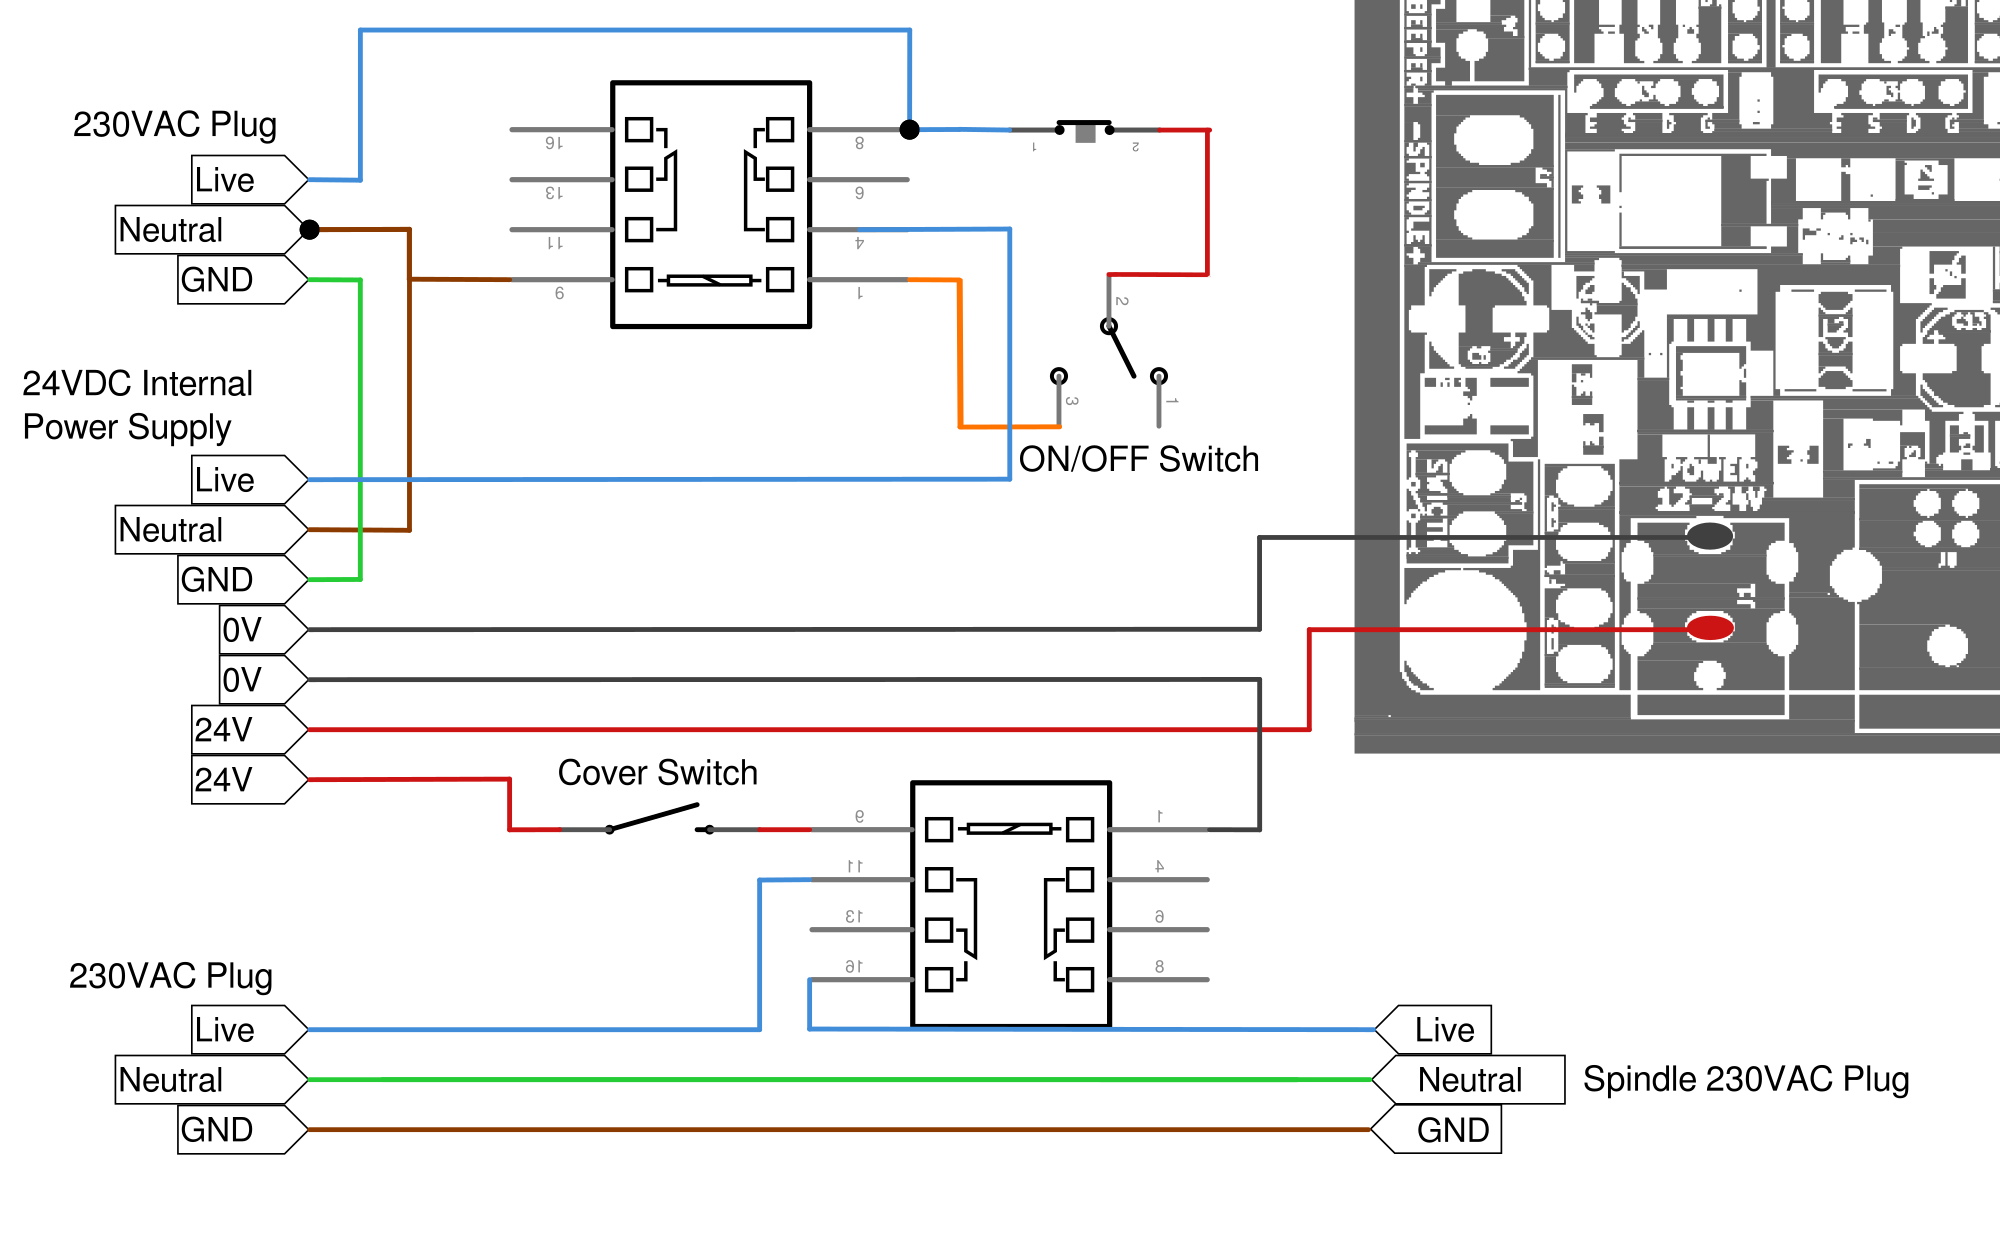
\includegraphics[width=0.8\textwidth]{./includes/schema_alim.png}
          \caption{Power circuit inside the machine }
      \end{figure}
    

      In the circuit above, the 230VAC is connected to connected to a a 230VAC relay which is controlled by the emergency stop button and the front panel switch. If the latter are closed the relay will be triggered and power will be supplied to the power supply which in turn powers the motherboard.
      
      The cable going from the power supply to the motherboard is custom-made and has been extended in order to reach the external module. The red wire is the 24VDC output and the yellow wire is the GND. 

      The cover switch is a magnetic contact sensor attached to the left side of the machine case and connected at the back of the machine on the \texttt{Capot} port. The switch is normally open and will close when the cover is lowered. 
      
      Internally the connector has been soldered in series with the \texttt{10A relay} port which powers the spindle control box. This way the spindle will only be powered when the cover is closed. The cable going to the spindle control box is a custom RCA to stereo jack adaptor which has been extended to reach the control box.

      Inside the spindle control box is a 24VDC relay which when triggered will close the circuit of the live wire to the spindle power socket. 

    \subsubsection{Control circuit}

        \begin{figure}[ht!]
            \centering
            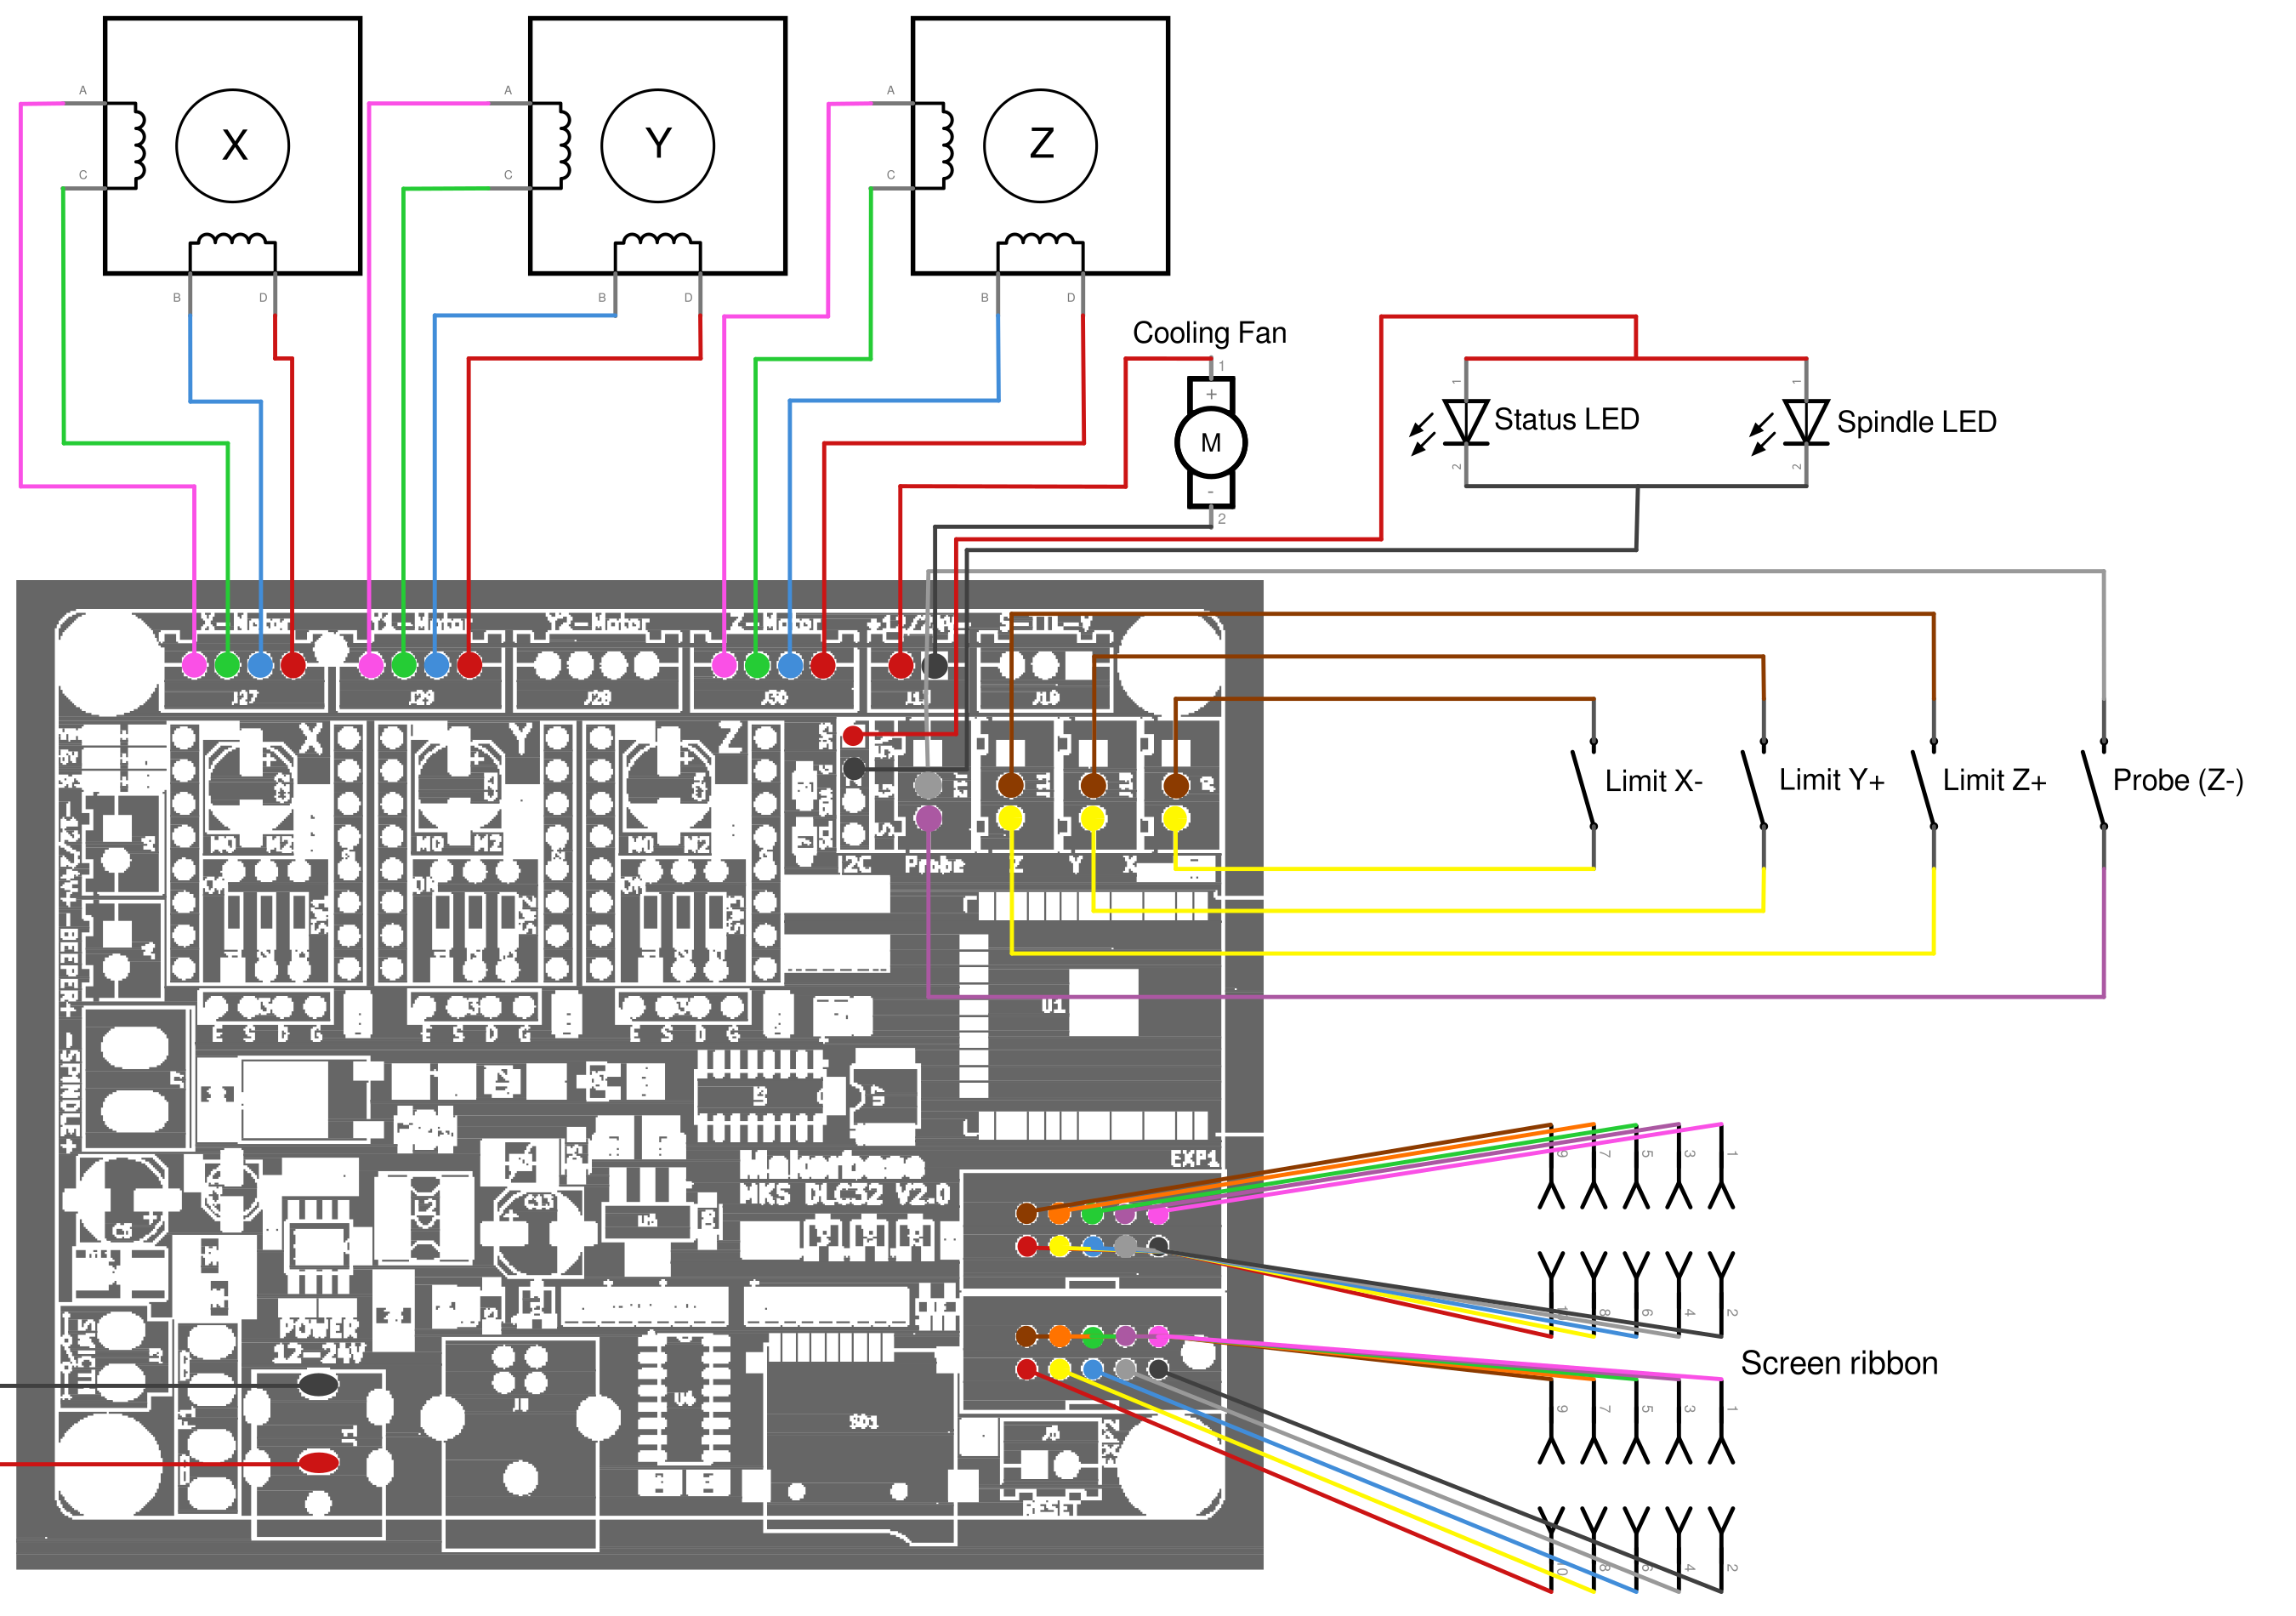
\includegraphics[width=0.8\textwidth]{./includes/schema_command.png}
            \caption{control circuit inside the external module }
        \end{figure}

    The 3 axes are controlled by stepper motors inside the machine that are connected to the CNC motherboard via custom-made cables these connect to the \texttt{X}, \texttt{Y1}, \texttt{Z} outputs of the shield. For each axis a \texttt{DRV8825} stepper driver is used to control the stepper motors, the Z-Axis drive being the only one missing a heat-sync.
    
    The axis cables contain 6 inner wires: 4 for the stepper motor (2 for each coil) and 2 for the limit switch. These limit switches are connected through a domino connector to the motherboard since the connectors themselves have unreliable connectivity issues. The Z-Axis cable contains an additional 2 wires for the spindle LEDs. 

    The wires of the spindle LED are interconnected with the status LED wires coming from the RJ45 cable in order to be in a parallel circuit. These cables are then connected to the motherboard on the 3.3V output and the GND pin of the I2C connector. 
     \begin{dent}{Note:}
        Because the wires of the status LED and spindle LED are interconnected and soldered, the Z-Axis cable and RJ45 cable are bound to each other.
    \end{dent}
    \vspace{5pt}

    The Z touch probe is connected to the motherboard through the RJ45 cable on the \texttt{Z-Probe} pins of the shield. The connectors are not custom-made, the connectivity is made with single strand female connectors.
     \begin{dent}{\textbf{Caution:}}
        Since this connection is made with single strand connectors, the connection is not reliable and can be easily disconnected. This connection should be checked after any handling of the shield.
    \end{dent}
    \vspace{5pt}

    To cool the stepper drivers a 12VDC/0.17A fan is placed inside the external module and is powered by the 24VDC output of the motherboard.

    The external module also contains a TS35 touch screen which is connected to the CNC motherboard through the \texttt{EXP1} and \texttt{EXP2} connectors. The touch screen is powered by the motherboard and displays the current machine status.


     \subsubsection{Complete Circuit}

        The complete circuit of the machine is shown below.

        \begin{figure}[ht!]
            \centering
            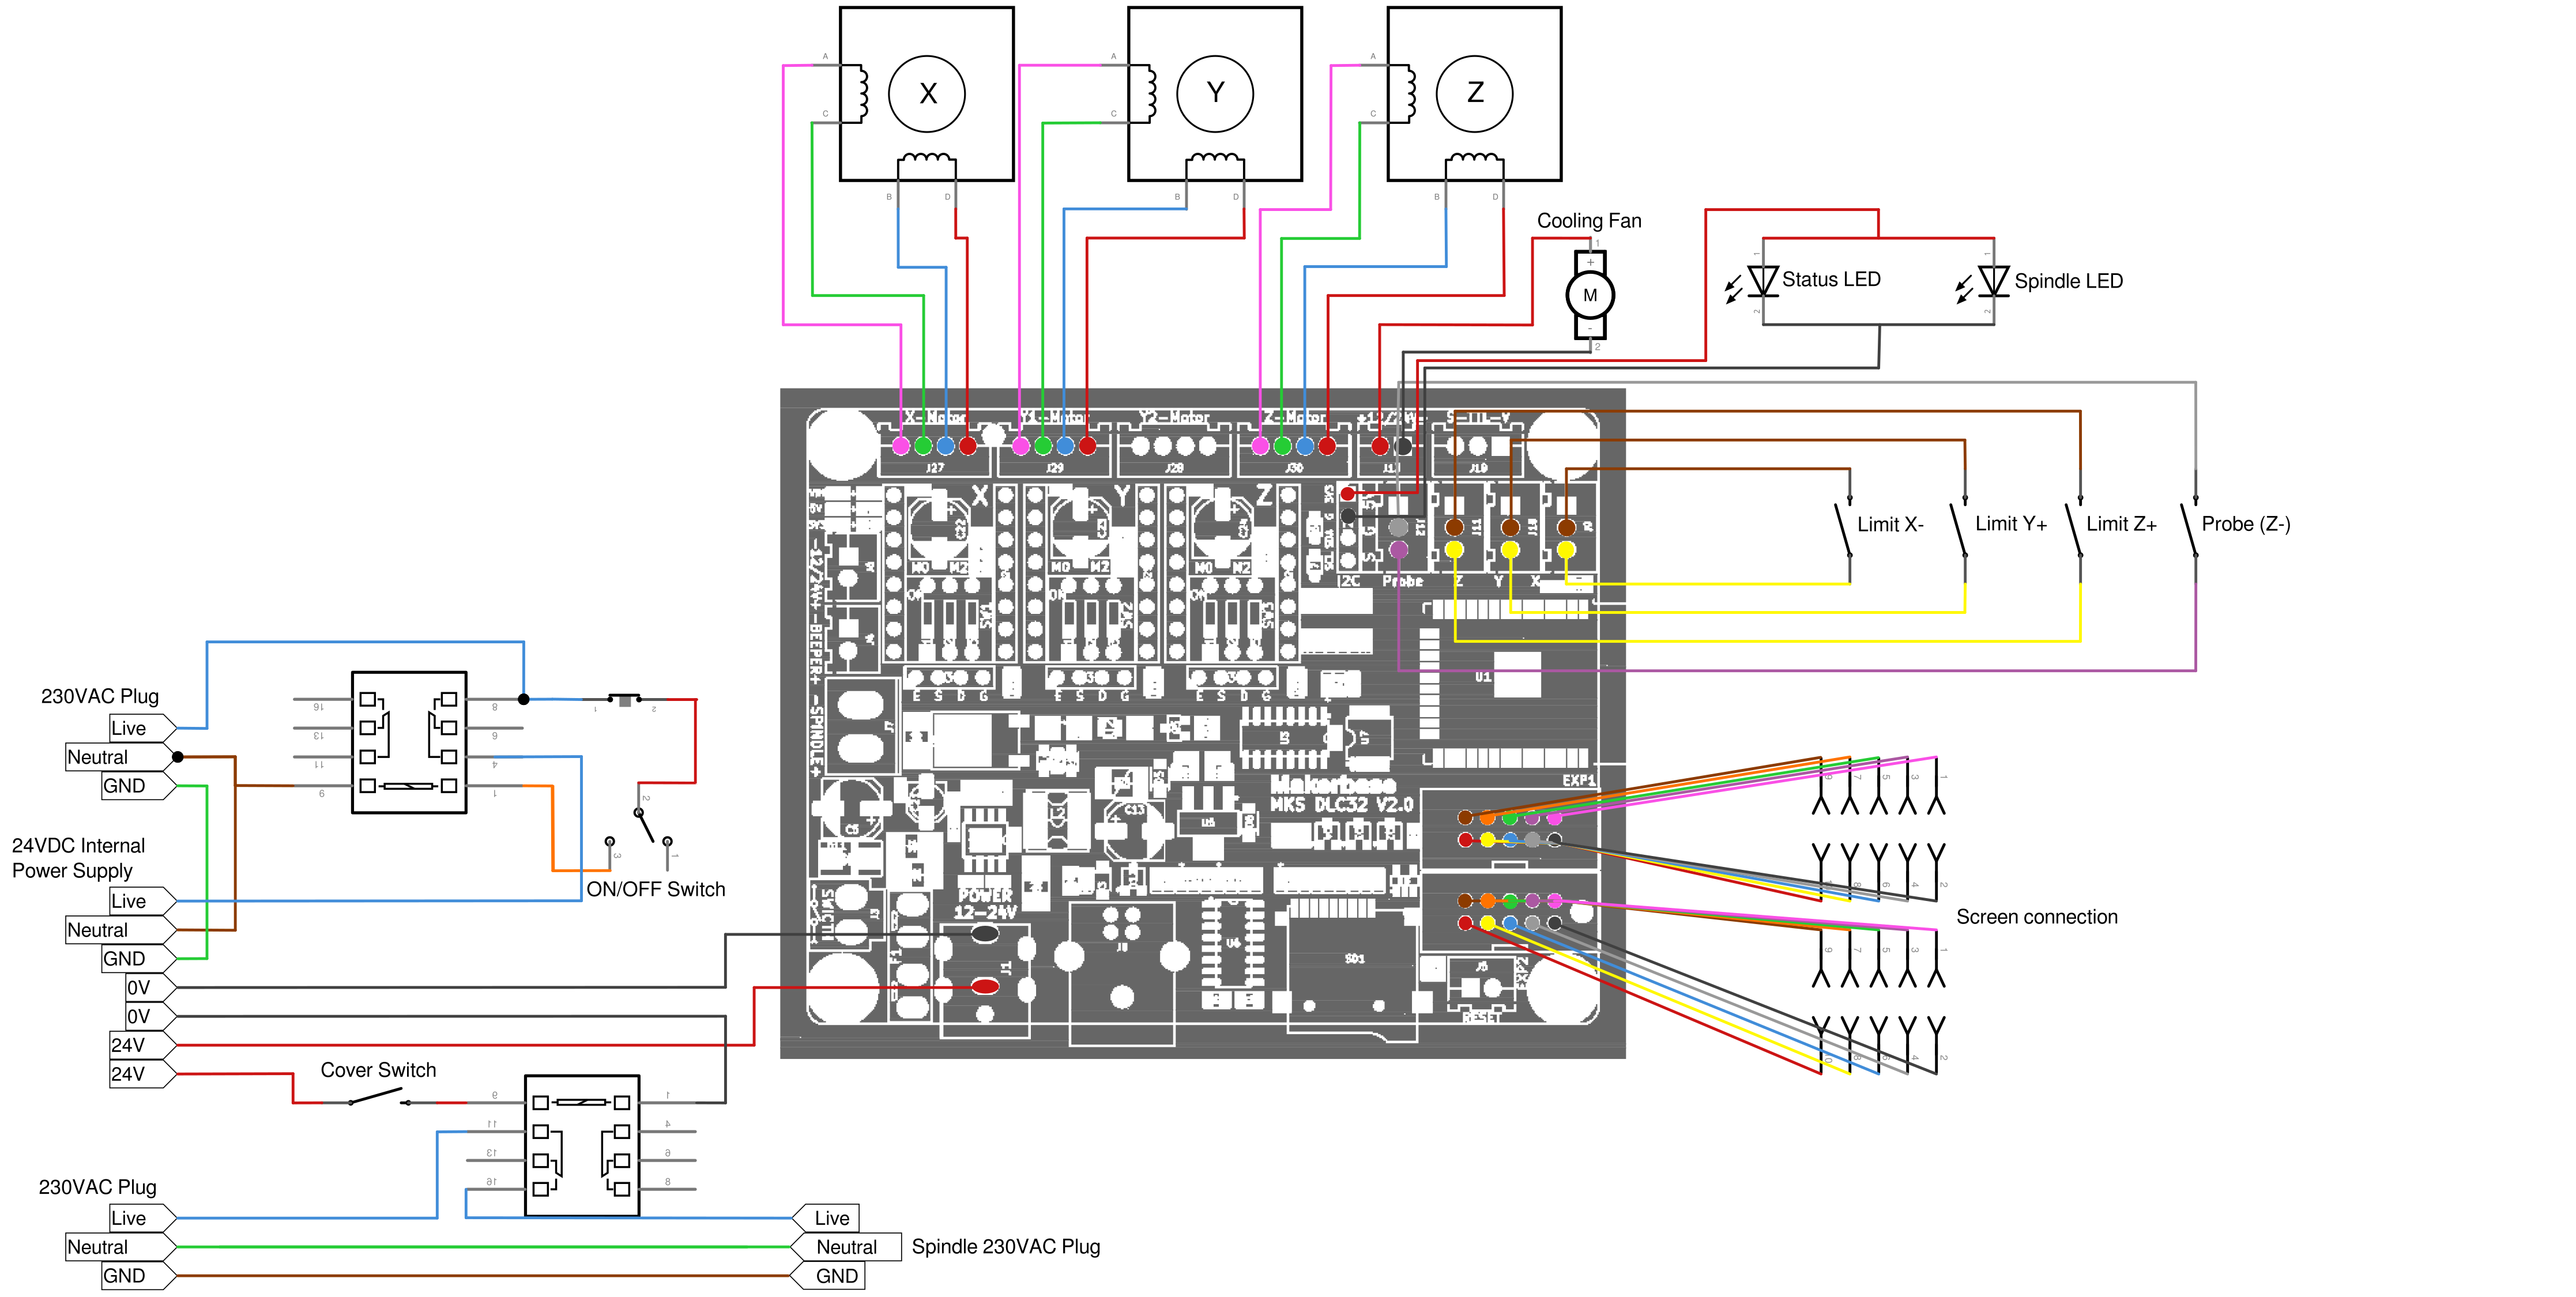
\includegraphics[angle=90, width=0.7\textwidth]{./includes/schema_global.png}
            \caption{Complete circuit of the machine}
        \end{figure}

        \newpage





    
    

    \section{Basic Control Operation}

         \subsection{Startup Procedure}

         Before starting, check that the front panel switch is in the OFF position and with its cap closed. To avoid powering the spindle, make sure the protective cover is \textbf{open}. 

         Plug the 230VAC power cable into the wall socket. Check that the emergency stop button is disengaged by twisting the button clockwise to release it. The machine in now ready to be powered on.

          \begin{dent}{\textcolor{red}{\textbf{WARNING:}}}
             After prolonged use of the machine or after reconfiguration of any machine component, including the external module, these guidelines must be followed.
             \textbf{Any deviation from the expected behavior must require a full review of the machine and its components.}

             \textbf{IF ANY OF THE AXIS START MOVING DURING THIS PROCEDURE IMMEDIATELY HIT THE EMERGENCY STOP BUTTON.}
         \end{dent}
         \vspace{5pt}

        To power on the machine flick the front panel switch cap to an open position. Then set the switch to the ON position. 
        
        A single clicking sound should be heard from the relays inside the machine. The machine should power on with a slight whizzing sound from the axis motors for a few seconds, but\textbf{ no movement should occur}. The status LED should light up along with the spindle LEDs. The external module cooling fan should also start spinning and the TS35 touchscreen should start up.

        Before using the machine, the user must ensure that the machine is in a safe state. Connect to the machine using the USB cable and open the CNCjs software. In the console the user must type '\texttt{\$> ?}'. This will display information about the machine's status, what should always be checked is if the any of the axis pins other than the Z-probe are triggered. 
         \begin{lstlisting}
<Idle|MPos:3.000,-3.000,-3.000|FS:0,0|Pn:P|WCO:97.000,-153.000,-30.966>
        \end{lstlisting}
        

        
        The pin field  should be \texttt{Pn:P}. \textbf{If this is not found or not the case, the machine is not in a safe state and should not be used.}
        
    \subsection{Manual Controls}

        When using manual controls the machine can be entirely controlled in an unrestricted manner. This means that the machine will ignore any physical limits and will move in the direction specified by the user. 

         \begin{dent}{\textbf{Caution:}}
            While in manual controls, the axis hard limits will only stop \textbf{a single instruction} from moving past physical limits. However if the user insists on moving the machine past these limits, the machine will do so \textbf{ignoring the hard limits.}
            \textbf{The user is responsible for the machine's movement and must be aware of the machine's position at all times.}
        \end{dent}

        \subsubsection{Touch screen}

        The touch screen is an interface that allows the user to control the machine. The screen contains 3 main pages: \texttt{Control}, \texttt{Sculpture} and \texttt{Tool}. 

        On the home page, the user can see the current machine working coordinates and mechanical coordinates. Since working coordinates are set only upon homing and Z-probing the machine, these values should not be considered accurate unless already done so.
        
        The \texttt{Control} page allows the user to manually control the machine. The user can move the machine in the X, Y, and Z directions by pressing the corresponding arrows. Pressing the home button for each axis moves the machine to the working coordinates home position. 
        \begin{dent}{\textcolor{red}{\textbf{WARNING:}}}
            \textbf{Do not press the home position button without having previsouly homed and Z-probed the machine.} 
        \end{dent}
        \vspace{5pt}
        On the right side of the \texttt{Control} page are different movement parameters that can be changed to control movement speed and distance increments(Speed control is not functionnal). The \texttt{Spindle} button is not functional since the spindle is not controlled by the motherboard.
        
        On the top part of the \texttt{Control} page the working coordinates are displayed together with a menu bar. The menu contains different functions some of which non-functional (\texttt{Knife} and \texttt{Cooling}). \texttt{XY\_Clear} will clear the XY working coordinates and set them to 0. \texttt{Z\_Clear} will clear the Z working coordinates and set them to 0. \texttt{HHome} will home the machine and recalibrate the mechanical coordinates. 

        The \texttt{Sculpture} page is not functional and should not be used.  


        The \texttt{Tool} page is used to access machine information, change the language of the machine or connect to an existing wifi. 

        \subsubsection{USB Connection}

        Numerical control by a computer is done through a USB cable connected to the motherboard. The CNC is recognized as a serial port and can be controlled by CNC milling software, such as \textbf{CNCjs}.
        
        Once connected to the machine using \textbf{CNCjs}, the machine does not yet know its current position. Any values displayed on the software interface or TS35 touch screen should not be considered accurate. 

        If the machine can not yet be controlled by the software. This means it is in a \texttt{lock state}. To remove this state, \texttt{\$X} must be typed in the machine console. This will unlock the machine and allow it to be manually controlled. Alternatively, the machine can be unlocked by pressing the \texttt{Reset} button on the software interface.
        
        \subsection{Automatic controls}

        To start an automatic control operation or a job the machine must first know its current position. This is done by homing the machine. Homing the machine can be done through the software interface (or in the console using \texttt{\$H}),  or through the TS35 touch screen in the \texttt{Control} page. 

        The machine should first rise on the Z-Axis and trigger the Z-Axis limit switch. Then move to the back left corner and trigger the X and Y-Axis limit switches independently.

         \begin{dent}{\textcolor{red}{\textbf{WARNING:}}}
                \textbf{BEFORE ANY OPERATION IS MADE THE MACHINE MUST BE HOMED.}

                \textbf{Due to the machine not knowing where it is, any movement can lead the machine to pushing past physical limits and may cause severe damage to its components.}
        \end{dent}

        Once the machine is homed the machine coordinates should update to $(3,-3,-3)$, both on the software interface and the TS35 touch screen. This however is insufficient since no information about the length of the spindle is known. 
    
        In order to calibrate the machine to the spindle height, a custom macro must be run by the software. The macro will use machine coordinates to place itself on top of the Z touch probe then lower itself slowly until the probe is triggered. The machine will then update its Z coordinate to the height of the spindle with a 1.5mm offset since the probe is triggered 1.5mm below the support plate.
        Soft limits in Z-Axis are also set to prevent the machine from moving past the support plate.

        Once this is done the machine will automatically go back to its mechanical home position and set the working coordinates of the machine to the center of the support plate. The machine is now ready to be used to start a job.

         \begin{dent}{\textcolor{red}{\textbf{WARNING:}}}
            \textbf{NEVER RUN THE Z PROBE MACRO WITHOUT HOMING THE MACHINE.}
            
            \textbf{The macro relies on machine coordinated to function correctly. If the machine coordinates  have not been correctly updated, the machine will not be aligned with the touch probe and may cause damage to the machine.}

        \end{dent}

        The macro code is given below:
         \begin{figure}[ht!]
         \begin{lstlisting}
; Remove soft limits
$20=0

; Place spindle above z-probe
G21
G53 G0 Z-3
G53 G0 X21.5 Y-16

; Z-Probe trigger search
G91
G38.4 Z-35 F200
G90

;Offset spindle height to plate height
G10L20 Z-1.3
;Set working coordinates
G10L20 X-75.5 Y137

; Retract from the touch plate and go to mechanical home position
G53 G0 Z-3
G53 G0 X3 Y-3
G4 P1
; Soft limit
$20=1
%Z0=posz+3
$132=[Z0]
        \end{lstlisting}
        \caption{Z-Probe Macro}
    \end{figure}




 \section{Circuit printing}

    Before any, and every, job is given through the software interface, the machine must be homed and Z-probed. This is to ensure that the machine knows its current position and can prevent any damage to its components.

     \begin{dent}{\textbf{Note:}}
        It is advised to move the machine to the woking home position before starting a job. 
    \end{dent}

    The job must be a G-Code file that is compatible with the machine. The maximum working area of the machine is 188x300mm, and the center of the support plate is the working origin of the machine. Soft limits are set to prevent the machine from moving past the support plate.

    When printing the design of a circuit, it should be noted that the $Z=0$ working coordinate can be offset above the support plate. Hence, with a 1.5mm thick copperboard, a 0.1mm deep cut can be equivalent to a cut height of 1.3mm($Z_{board}- Z_{offset} - Z_{cut}$). Through testing we found the optimal cut depth to be no more than 0.2mm, any deeper can damage the drill piece. 

     \subsection{G-Code files and GERBER conversion}

    To print a circuit we recommend using \texttt{Fusion 360} which can directly export a project to a G-Code file. \texttt{GERBER} files can also be used but must first be converted to a G-Code file.

    Since most electronic circuit design software can export to a GERBER file, we will details the steps to convert a GERBER to G-Code using FlatCAM (\textbf{version 8.4}\footnote[1]{Version 8.4 allows for adjustable cut height above 0, others do not}).

   
    
     \begin{figure}[ht!]
        \centering
        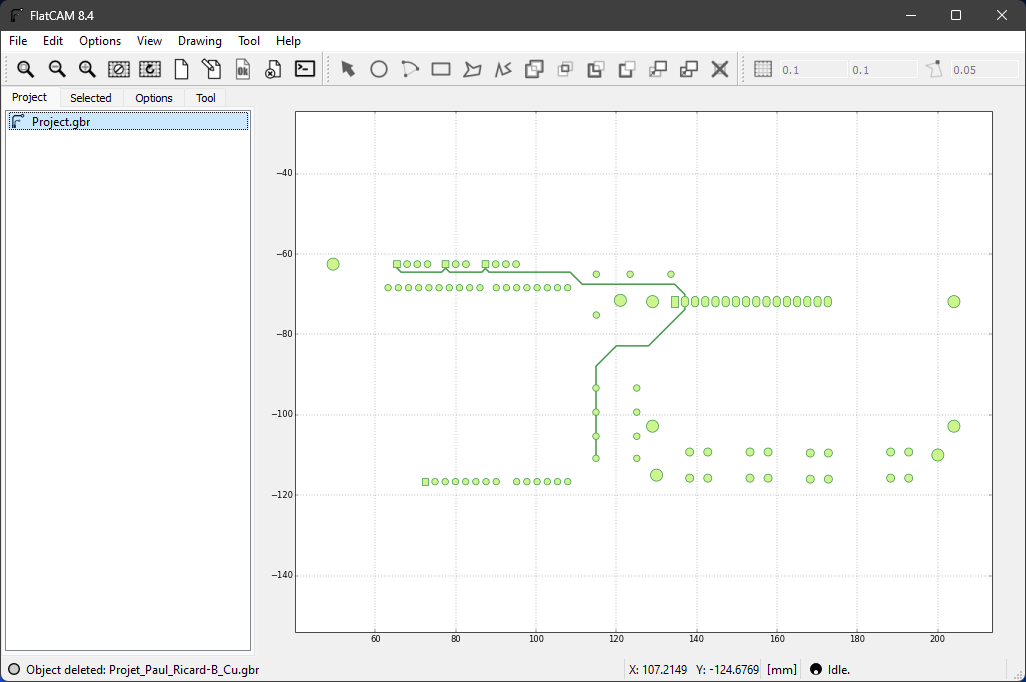
\includegraphics[width=0.8\textwidth]{./includes/G1.png}
        \caption{Project tree after importing the GERBER file}
    \end{figure}
    
    On figure 4.1 in the expected project tree after importing the GERBER file to FlatCam. The file should open with the expected cut shape and the toolpath should be visible.

    Double clicking on the GERBER file will open the geometry editor. This is how the cutout of the circuit is defined. Here the tool diameter should be specified depending on the dimension of the drill piece used. The \texttt{Width} parameter is used to extended the cutout to a bigger width, to do so the drilling piece make a second path over the entire geometry with a certain percentage of overlap. This can be usefull if the specified cutout is not wide enough for reliable soldering. 

    \begin{figure}[ht!]
        \centering
        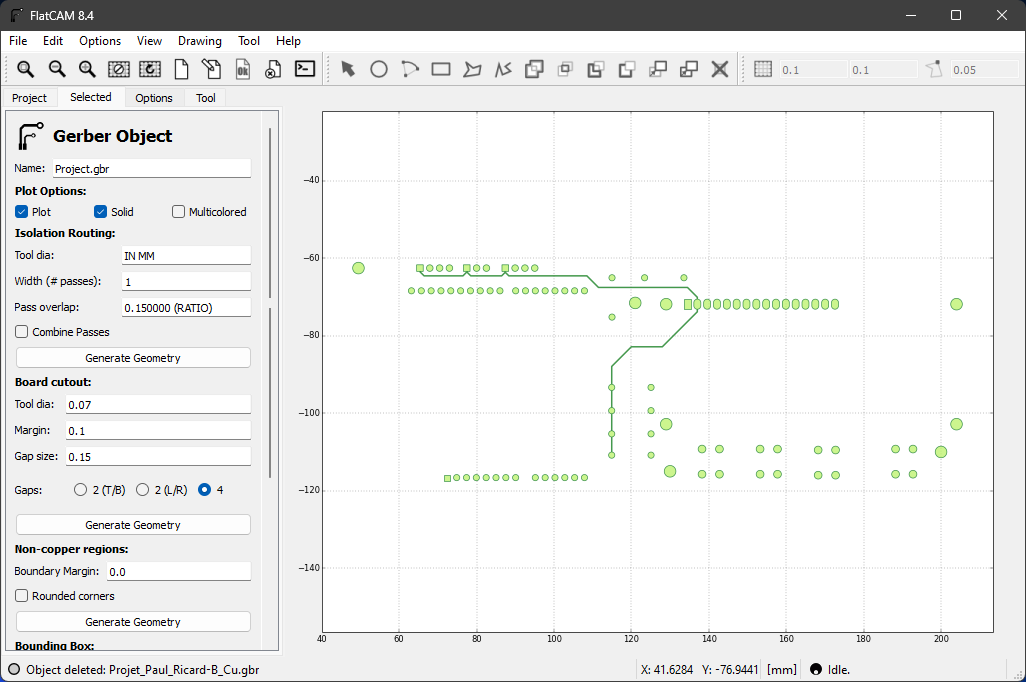
\includegraphics[width=0.8\textwidth]{./includes/G2.png}
        \caption{Geometry parametrisation of the cut}
    \end{figure}

    At the bottom of the geometry editor you can find an offset parameter which can help you center the cut of the circuit on the support plate. We recommend the preoject alway be at the center since the working coordinates are set to the center of the support plate.  

    After clicking \texttt{Generate Geometry} under the plot options scetion, the desired cutout should be seen in red and a new geometry file is created in the project tree. Double clicking on this file will open the cutting parameters. 

    \begin{figure}[ht!]
        \centering
        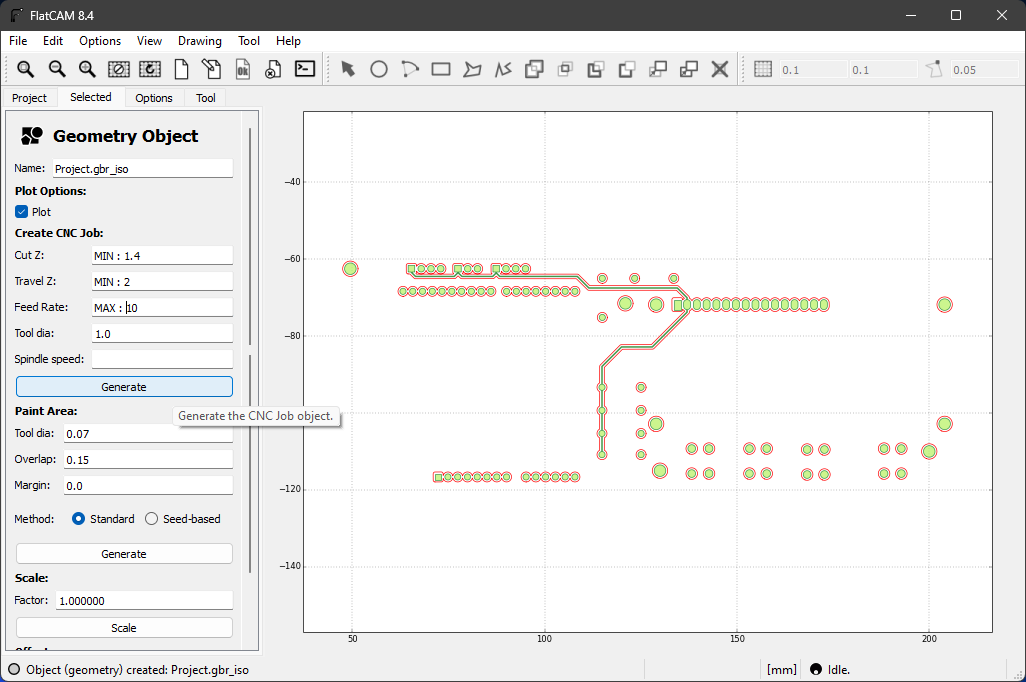
\includegraphics[width=0.8\textwidth]{./includes/G3.png}
        \caption{Cutting parameters}
    \end{figure}

    This tab allows the user to select the cutting parameters that will be passed to the machine, and is thereby the most dangerous part of this process. \textbf{A wrong parameter can lead to a broken drill piece or a damaged machine.}

    \texttt{Cut Z} defines the Z-height at which the cut will be made.
    $Z_{height}=Z_{board}-Z_{cut}$ where the $Z_{cut}$ is the value of the cut depth which we recommend should not exceed 0.2mm. $Z_{height}$ should be around 1.4mm.  

    \texttt{Travel Z} defines the Z-height at which the machine will move between cuts. This should be set to a value higher than the board height to avoid damaging the drill piece. We recommend a height of 2mm. 

    \texttt{Feedrate} defines the speed at which the machine will move during cutouts. This should be set to a value that is not too high to avoid damaging the drill piece. We recommend not exceeding a value of 7mm/min, but this can be adjusted based on the sturdiness of the drill piece used.



     \begin{figure}[ht!]
        \centering
        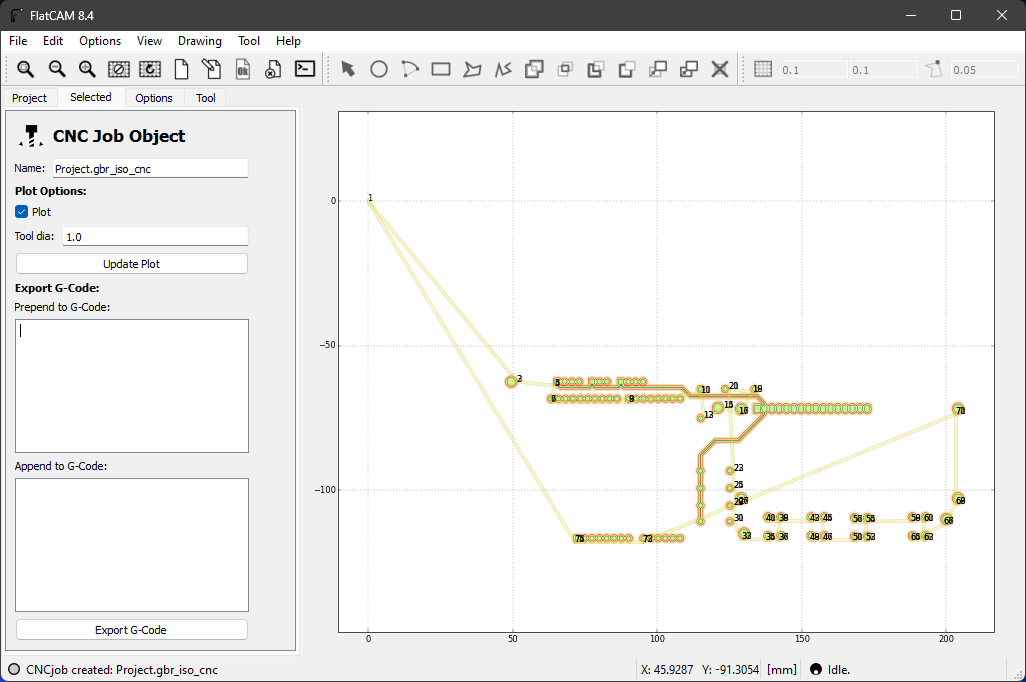
\includegraphics[width=0.8\textwidth]{./includes/G4.png}
        \caption{CNC job file, and toolpath}
    \end{figure}

    Once this has been set and the plot options have been set and generated, A CNC job file will be generated. You can check here if the toolpath is correct and if the cutout is as expected, especially near small cutting gaps where the tool diameter set may not be able to fit.

    The generated job can then be exported when double clicking on the job file. The resulting G-Code file can then be sent to the machine through the CNCjs software interface. 

    \begin{dent}{\textbf{Caution:}}
        At the start of any job please keep a hand ready on the emergency stop button in case the print parameters have been set incorrectly.
    \end{dent}    


    




 \section{Maintenance and Troubleshooting}

    \subsection{Maintenance checks}

    The machine should be regularly inspected for any signs of wear, damage, or malfunction. The following maintenance checks should be performed on a regular basis:

    \begin{items}[-3pt]{-15pt}{-15pt}
        \item Check the limit switches for proper operation. The switches should trigger when the machine reaches its physical limits.
        \item Check the spindle control box for any signs of damage or malfunction. The spindle should only be powered when the protective cover is closed.
        \item Check the external module cooling fan for proper operation. The fan should be spinning when the machine is powered on and with sufficient airflow to cool the drivers.
        \item Check the Z touch probe for proper operation. The probe should trigger when the machine reaches the top of the support plate.
        \item Check the front panel power switch and emergency stop button for proper operation. The machine should only be powered on when the front panel switch is in the ON position and the emergency stop button is disengaged.
    \end{items}

    If any signs of wear, damage, or malfunction are found during the inspection, the machine should be powered off and a qualified technician should be contacted for further assistance.

    Regularly grease the axis rails. The grease should be applied to the rails and the moving parts of the machine. The machine should be powered off before applying the grease.


     \subsection{Maintenance disasembly}

    The machine can be disassembled for maintenance purposes. The following steps should be taken to disassemble the external module or the machine. 

     \subsubsection{External module}

     Unslide the screen font panel, and detach the \texttt{EXP1} and \texttt{EXP2} connectors.

     The inside should be a rat's nest of cables. First remove the Z-probe, LED and fan cables from the motherboard. 
     
     Then remove the axis cables from the motherboard. Do not pull on them forcefully since the RJ45 cable is linked to the Z-Axis cable, and each cable contains the limit switch wires.

     Remove the limit switch cables from the domino connector. Avoid moving the board connectors as they are not reliable.

     Disconnect the power supply cable from the motherboard.

    The external module can now be removed from the machine.


     \begin{dent}{\textbf{Note:}}
        To reassemble the external module, follow these steps in reverse order. Make sure that all cables are properly connected and secure before powering on the machine. Then perform maintenance checks and startup procedures as outlined in this manual.
    \end{dent}

    \subsubsection{Machine}

    The front panel of the machine can be disassembled by removing the screws on the front panel. Inside is the circuitry of the front panel switch and emergency stop button as well as the status LED and Z-Probe switch which are contained in the RJ45 cable.

    The spindle control box can be disassembled by removing the screws on the control box. Inside is the relay that controls the spindle power. The relay should be checked for proper operation and any signs of damage.

    On the back panel of the machine is the contact sensor's cable which can be simply unplugged.

    To acces to the insides of the machine the right side panel should be unscrewed and carefull removed together with the top panel. 


    \subsection{Troubleshooting}

     Review the machine's status in the software interface using \texttt{\$> ?} to check if the machine is in a safe state. And if the machine is properly configured using \texttt{\$> \$\$}. 

    If the machine is not operating as expected during maintenance checks, we provide the following troubleshooting assistance based on our experience with the machine: 

     \subsubsection{Machine not powering on}
     
     If the PSU doesn't power on when the front panel switch is set to ON, check the relay and circuitry inside the machine against the provided electrical documentation. The relay should trigger when the front panel switch is set to ON and the emergency stop button is disengaged. In the case where the relay is not triggered, the front panel switch or emergency stop button may be faulty.
     
     If the PSU powers on but the external module does not, first check that the power cable is properly connected to the motherboard. If the external module still does not power on, open the machine and check the connections and soldering of the 24V output cable to the back panels ports. 

      \subsubsection{Axis not moving when commanded}

        If the axis does not move when commanded through the software interface or the touch screen, check the connections between the motherboard and the stepper drivers.

        Additionally check the status of the limit switches, if any of the switches seem faulty, this could be due to the unreliable connection to the moetherboard. We recommend applying a small amount of pressure on the pins to ensure a proper connection (and slightly wiggle if this does not work). 

        If the problems lies with the Z-Axis, the 3 pin connector of the Z-Probe should be replaced properly to ensure that the connection is reliable.

     \subsubsection{Touch Z-probe not triggering}

        If the Z touch probe does not trigger when the button is pressed down, check the cable connection to the motherboard, and inside the front panel on the domino. 

        If the probe is stuck, then the support plate should be carefully removed. Underneath it the switch must be removed and the button should be pushed back up. 

      \subsubsection{The spindle powers on when the cover is open}

        If the spindle powers on when the cover is open this can be due to the ferromagnetic property of the cage which is strong enough to trigger the contact sensor, however the precise reason is unknown. 

        To fix this we recommend removing the contact sensor from the cage and placing it outside of a few minutes to reset the sensor. Additionally the protective cover should not be toyed around with since this problem has been noticed to happen when the contact sensor commutates too fast. 
        
        The sensor should close when the cover is lowered (the relay inside the spindle control box should be heard triggering).  
  

       If the machine is still not operating as expected after performing these troubleshooting steps, the machine should be powered off and a qualified technician should be contacted for further assistance.

       \subsection{Configuration parameters}

         The machine configuration can be accessed through the software interface using \texttt{\$> \$\$}. Do not modify these values as they can compromise safety of the equipment. The following parameters are used to configure the machine:
 
\footnotesize
          \begin{lstlisting}
$0=10 (Step pulse time, microseconds)
$1=25 (Step idle delay, milliseconds)
$2=0 (Step pulse invert, mask)
$3=6 (Step direction invert, mask)
$4=0 (Invert step enable pin, boolean)
$5=0 (Invert limit pins, boolean)
$6=1 (Invert probe pin, boolean)
$46=10.000
$10=1 (Status report options, mask)
$11=0.010 (Junction deviation, millimeters)
$12=0.002 (Arc tolerance, millimeters)
$13=0 (Report in inches, boolean)
$20=1 (Soft limits enable, boolean)
$21=1 (Hard limits enable, boolean)
$22=1 (Homing cycle enable, boolean)
$23=1 (Homing direction invert, mask)
$24=300.000 (Homing locate feed rate, mm/min)
$25=1000.000 (Homing search seek rate, mm/min)
$26=250.000 (Homing switch debounce delay, milliseconds)
$27=3.000 (Homing switch pull-off distance, millimeters)
$28=1920.000
$30=10000.000 (Maximum spindle speed, RPM)
$31=0.000 (Minimum spindle speed, RPM)
$32=0 (Laser-mode enable, boolean)
$38=1
$40=1
$100=800.000 (X-axis travel resolution, step/mm)
$101=800.000 (Y-axis travel resolution, step/mm)
$102=800.000 (Z-axis travel resolution, step/mm)
$103=100.000
$104=100.000
$105=100.000
$110=1000.000 (X-axis maximum rate, mm/min)
$111=1000.000 (Y-axis maximum rate, mm/min)
$112=1000.000 (Z-axis maximum rate, mm/min)
$113=1000.000
$114=1000.000
$115=1000.000
$120=500.000 (X-axis acceleration, mm/sec^2)
$121=500.000 (Y-axis acceleration, mm/sec^2)
$122=500.000 (Z-axis acceleration, mm/sec^2)
$123=200.000
$124=200.000
$125=200.000
$130=188.000 (X-axis maximum travel, millimeters)
$131=300.000 (Y-axis maximum travel, millimeters)
$132=30.966 (Z-axis maximum travel, millimeters)
$133=300.000
$134=300.000
$135=300.000
         \end{lstlisting}




        




















    

\end{document}